\documentclass[12pt,a4paper]{article}
\usepackage[top=25.4mm, bottom=25.4mm, left=19.1mm, right=19.1mm]{geometry}


\usepackage[latin2]{inputenc}
\usepackage{graphicx}
\graphicspath{ {./images/} }
\usepackage{ulem}
\usepackage{amsmath}
\usepackage[document]{ragged2e}

\setlength{\parindent}{4em}
\setlength{\parskip}{1em}
\usepackage{hyperref}

\usepackage{fancyhdr}
\pagestyle{fancy}
\fancyhf{}
\fancyhead[LO]{\textbf{\small IoT and Smart Analytics}\\
\text{\small A Program by IIITH and TalentSprint}}

\usepackage{xcolor}
\usepackage{lipsum}

\rhead{\begin{picture}(0,0) \put(-250,-2){
\includegraphics[width=9cm]{EXP_08_Images/ts-iisc-logo-pr.png}} \end{picture}}
\cfoot{\thepage}


\begin{document}

\begin{center}

\textbf{\large \\EXPERIMENT 07 }\\[6pt]
\text{Arduino Interfacing with LM35 and LDR }
\end{center}

\textbf{\large LEARNING OBJECTIVES:}\\[3pt]
At the end of this experiment, participants will be able to:\vspace{-6mm}\begin{enumerate}
 \setlength\itemsep{-0.3em}
\item Connect \& use LM35 temperature sensor with Arduino  \\
\item Connect \& use LDR with Arduino \\
\item Understand \& use external/internal analog  reference voltages in Arduino 
\end{enumerate}
\textbf{\large APPARATUS REQUIRED:}\\
\vspace{-3mm}
\begin{enumerate}
 \setlength\itemsep{-0.3em}
\item Arduino Module-1pcs \\
\item USB cable-1pcs\\
\item Arduino IDE
\item Breadboard-1pcs\\
\item LM35-1pcs\\
\item LDR-1pcs\\
\item LED-1pcs\\
\item Resistor 1k$\Omega$ -1pcs\\
\item Jumper wires\\

\end{enumerate}

\begin{justify}
\textbf{\large THEORY}\\[3pt]
\textbf{LM35:} The LM35 is a linear temperature sensor whose output voltage varies linearly with temperature changes and gives analog output. The voltage output of the LM35 increases by 10mV per degree Celsius rise in temperature. It can measure temperature from-55 degrees celsius to +150 degrees celsius.  LM35 can be operated from a 5V supply and the standby current is less than 60uA. It has three terminals as shown in the figure below.

\begin{center} 
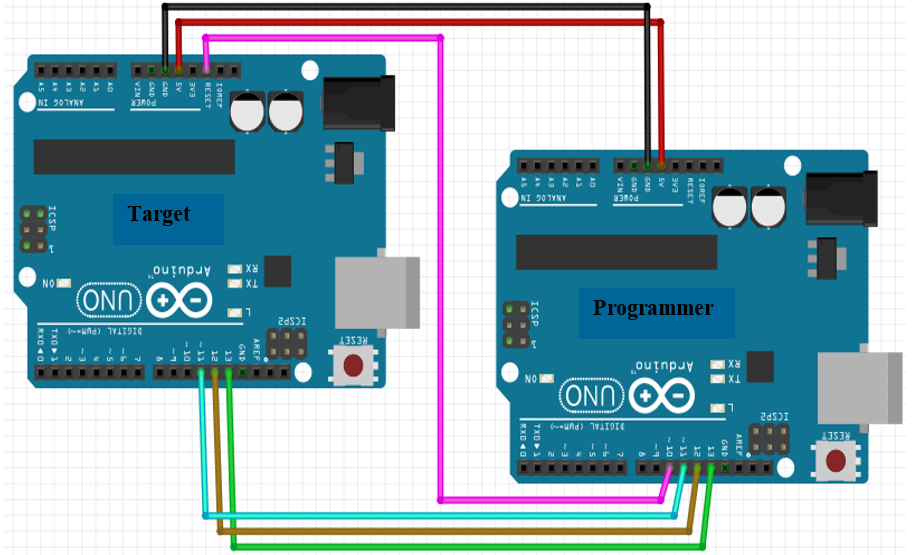
\includegraphics[scale=0.5]{EXP_07_Images/fig1.png}
\end{center}

\begin{center} {Figure 1. LM35 image and pinout}\end{center}

\noindent \textbf{Light Dependent Resistor (LDR): }These are resistors made up of a material (most commonly used: Cadmium Sulfide) whose resistance decreases with an increase in light incident on it (i.e., increasing illumination). Fig. 3  shows the characteristics curve of an LDR.

\begin{center} 
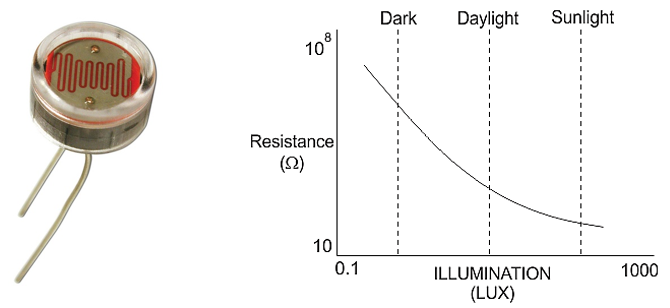
\includegraphics[scale=0.7]{EXP_07_Images/fig2_3.png}
\end{center}

\begin{center} {Figure 2. Image of an LDR [1] \hspace{12pt}   Figure 3. Characteristics of  an LDR [2] }\end{center}\\[21pt]

\noindent \textbf{\large PROCEDURE}\\[3pt]
\textbf{(A)	Interfacing LM35 with Arduino}\\[3pt]
\textbf{Hardware and software setup : }We can connect the hardware the same as in the TinkerCAD diagram given below. The Vcc terminal and the GND  of the LM35 (as shown in fig. 1) are connected to the 5 V and GND of the Arduino respectively. The mid terminal i.e Vout is connected to the analog pin A0.

\begin{center} 
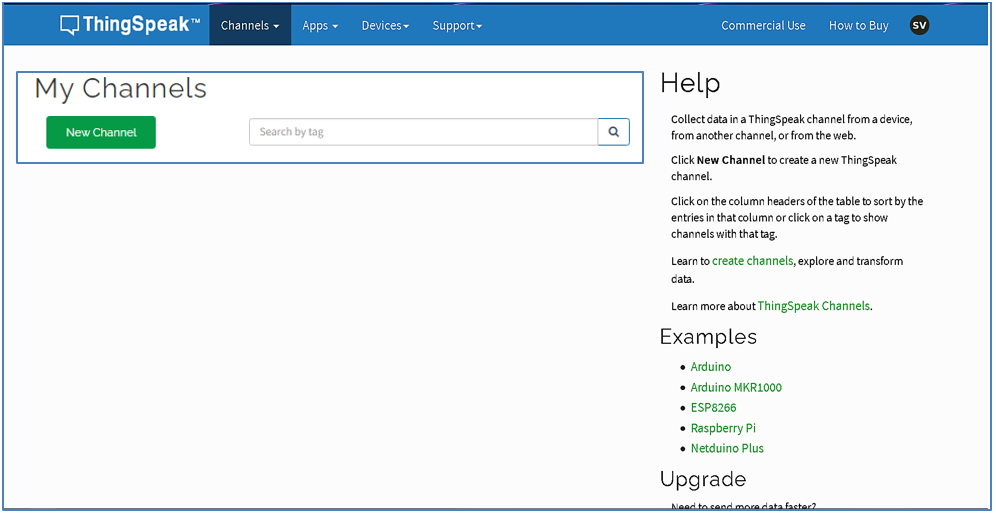
\includegraphics{EXP_07_Images/fig4.PNG}
\end{center}

\begin{center} {Figure 4. IThe hardware setup of LM35 with Arduino}\end{center}

\noindent Note: AREF is connected to 3.3V since we are going to use an external analog reference. For internal analog reference, we will not have any extra connection like this.\par
\noindent Normally, analog to digital converter in the Arduino uses the supply voltages of 5 Volts, and being  10-bit ADC there are 1024 individual steps that it can read in between 0 and 5 volts. But mostly, the sensor is not going to put out anywhere near 5 Volts, so analog reference voltage is used to change the sensor to read between 0 to 3.3 volts. Using reference voltages helps us to get higher accuracy, and now there will be 1024 steps in between 0 and 3.3 volts.
\end{justify}

\hspace{2cm}\textbf{\large Code:}\\[6pt]


\setlength{\parindent}{10eM}

\#define AREF\_Volt  3.3  \hspace{12pt}\textcolor{blue}{//Analog Reference voltage,\\ //The value will change for internal ref. see ref. [3]  }\\

int tempPin = 0; \hspace{12pt}\textcolor{blue}{// Connect TMP35 to Analog pin 0}\\
int tempRead; \hspace{12pt}\textcolor{blue}{// Analog tempereature result }\\[12pt]   

  void setup() \\
  \{\\
  Serial.begin(9600);\hspace{12pt}\textcolor{blue}{  // Initializing Serial Monitor} \\
  analogReference(EXTERNAL);\hspace{12pt}\textcolor{blue}{ // Ext. Analog Ref. voltage is used\\ // For internal ref. pass'INTERNAL' inside parenthesis}\\
\}\\[12pt]

void loop() \\
\{  \\                  
  tempRead = analogRead(tempPin); \hspace{12pt}\textcolor{blue}{// Read voltage value from\\ sensor// direcltyly 'A0' can be passed instead of 'tempPin'}\\
  Serial.print("Raw input : ");\hspace{12pt}\textcolor{blue}{// Print to serial monitor}\\
  Serial.print(tempRead); \\
  float voltage = (tempRead * AREF\_Volt)/1024.0;\\ \hspace{12pt}\textcolor{blue}{// Convert to voltage}\\
  Serial.print(" equivalent to : ");\hspace{12pt}\textcolor{blue}{ // Print voltage to serial monitor}\\
  Serial.print(voltage);\\
  Serial.println(" volts ");\\

  \textcolor{blue}{/*Convert from 10 mv per degree with 500 mV \\offset
  to degrees celsius((voltage - 500mV) * 1000/10) */ }\\

  float temp\_in\_C = (voltage - 0.5) * 1000/10 ; 
  \textcolor{blue}{// for LM35 simply \\: float temp\_in\_C = voltage * 1000/10} \\
  
  Serial.print("Temp. Reading = ");\hspace{12pt}\textcolor{blue}{//Print the temperature reading} \\
  
  Serial.print(temp\_in\_C);\\
  
  Serial.print("\xc2\xb0 ");\hspace{12pt}\textcolor{blue}{// for getting degree symbol}\\
  
 Serial.println("C\n");\\
 
  delay(2000);\\
\}

\noindent Note: Above code is written for  temperature sensor TMP36 available in TinkerCAD. But everything remains the same for LM35 as well with minor changes in the code as written in the comment above.
\vspace{20mm}


\setlength{\parindent}{0pt}

\begin{justify}
\textbf{(B) Interfacing LDR with Arduino}\\[3pt]
\textbf{Hardware and software setup :} We can connect the hardware the same as in the TinkerCAD diagram given below. LDR is connected to 5V and GND of Arduino through a resistor. One terminal of LDR is connected to analog pin A0. LED is connected to pin 13.\par
\noindent As light incident on the LDR changes, the resistance changes, and the corresponding voltage drop across the LDR also changes. The voltage drop across LDR is fed to A0. Based on a particular value of analog read, the LED glows.\end{justify}

\begin{center} 
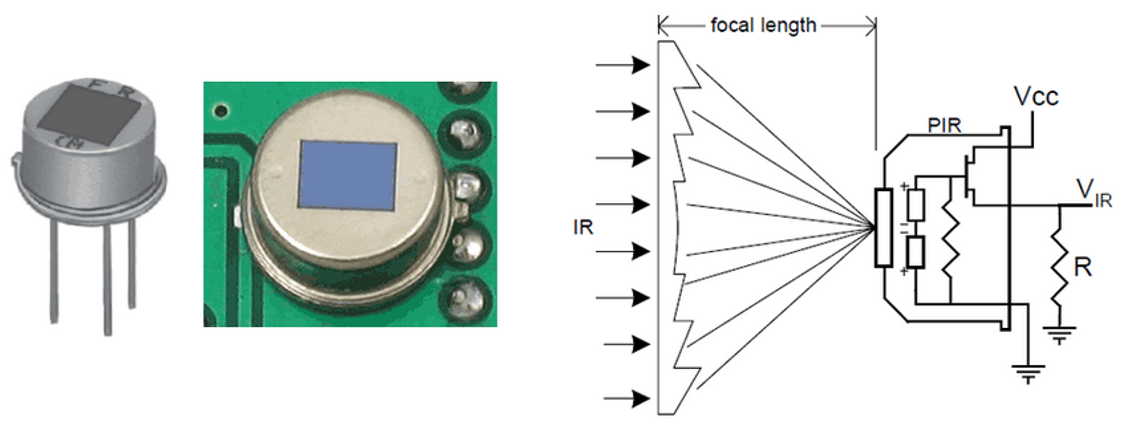
\includegraphics{EXP_07_Images/fig5.png}
\end{center}
\begin{center} {Figure 5. The hardware setup of LDR with Arduino}\end{center}
\vspace{10mm}
\hspace{2cm}\textbf{\large Code:}\\[6pt]

\setlength{\parindent}{10eM}

int value;\hspace{12pt}\textcolor{blue}{// variable for storing ouput of LDR through analog read}\\
int ledpin=13;\hspace{12pt}\textcolor{blue}{// Connected to LED}\\

void setup()\\
\{\\
   pinMode(ledpin, OUTPUT);\\
 Serial.begin(9600);\\
\}\\
\vspace{20mm}
void loop()\\
\{\\
  value=analogRead(A0);\\
 Serial.println(value); \hspace{12pt}\textcolor{blue}{ /*  Definining a condition, based on a particular\\ magnitude of 'value'.LED glows only for any value below/above \\that particular magnitude  */}\\

  if ( value $<$ 400)\{\\
  digitalWrite(ledpin, HIGH);\\
 \}\\
  else \{\\
    digitalWrite(ledpin, LOW);\\
  \}\\
  delay(1000); hspace{12pt}\textcolor{blue}{// Wait for 1000 millisecond(s)}\\

 \}\\[21pt]


\setlength{\parindent}{0eM}
\textbf{\large REFERENCES:}
\vspace{-6mm}
\begin{enumerate}
\setlength\itemsep{-0.3em}
\item  \href {https://engineershub.co.in/light-dependent-resistor-working-principle-and-its-applications/}{LDR : Working principle}
\item  \href {https://www.electrical4u.com/light-dependent-resistor-ldr-working-principle-of-ldr/}{LDR : Characteristics}
\item  \href {https://www.arduino.cc/reference/en/language/functions/analog-io/analogreference/}{Analog reference}
\end{enumerate}

\textbf{\large CONCEPT DRILLS:}
\vspace{-6mm}
\begin{justify}
\begin{enumerate}
 \setlength\itemsep{-0.3em}
\item Design a circuit and write the appropriate program (code) to generate different tones from a buzzer as the different intensity of light incident on the LDR connected with Arduino. The sound of different tones/frequencies is generated by changing the delay time between two buzzing. We can use a built-in function: 'Tone', available in Arduino.
\item Design a circuit and write the appropriate program (code) to trigger a buzzer below/above a certain temperature sensed by LM35. 
\end{enumerate}
\end{justify}

\end{document}